\documentclass{article}
\usepackage[utf8]{inputenc}
\usepackage{amsmath}
\usepackage{graphicx}

\title{Overview of Statistical Tests, P-values, and Confidence Intervals}
\author{}
\date{}

\begin{document}

\maketitle

\section{Statistical Tests}

Statistical tests are utilized to infer or draw conclusions about populations based on sample data. These can be classified into two main types: parametric and non-parametric. Parametric tests assume that data follows a specific distribution, whereas non-parametric tests do not. Examples include t-tests, chi-square tests, and ANOVA, chosen based on the research question, data type, and its distribution. 

\section{P-values}

The p-value quantifies the probability of observing a test statistic as extreme as, or more extreme than, the observed statistic under the assumption that the null hypothesis $H_0$ is true. It is defined as:
\[ p\text{-value} = P(T \geq t | H_0) \]
where $T$ is the test statistic and $t$ is the observed value. A p-value less than a pre-determined significance level, commonly $0.05$, suggests significant evidence against $H_0$, favoring the alternative hypothesis $H_a$. The significance level is arbitrarly chosen and limits the type-I error, falsely rejecting $H_0$ even though $H_0$ is true.

\section{Confidence Intervals (CIs)}

A confidence interval provides a range of values, expected to contain the true population parameter with a certain level of confidence (typically 95\%). The formula for a CI depends on the parameter being estimated but generally takes the form:
\[ \text{CI} = \text{estimate} \pm (\text{critical value}) \times (\text{standard error}) \]
CIs offer insights into the effect size and its precision. An interval that does not include the null value indicates statistical significance.

\section{Relationships}

\subsection{Statistical Tests and P-values}
Statistical tests yield a test statistic, leading to the calculation of a p-value, which quantifies the evidence against $H_0$. A small p-value indicates that the observed results are rare under $H_0$.

\subsection{Statistical Tests and CIs}
Statistical tests often result in an estimate and its CI, providing a range of plausible values for the population parameter. \textbf{If a CI does not include the value of $H_0$, it suggests a significant effect.}

\subsection{P-values and CIs}
While p-values indicate the existence of an effect, CIs describe the size and precision of the effect. \textbf{A significant p-value corresponds to a CI that does not include the null effect value.}

\section{Understanding Type I and Type II Errors and Power Curves in Hypothesis Testing}
\subsection{Type I and Type II Errors}
\subsubsection{Definitions}
A Type I error, also known as a false positive, occurs when the null hypothesis is true, but is erroneously rejected by the statistical test. The probability of committing a Type I error is denoted by the significance level, $\alpha$, which is predetermined by the researcher. Conversely, a Type II error, or a false negative, occurs when the null hypothesis is false but is erroneously accepted. The probability of a Type II error is denoted by $\beta$.
\subsubsection{Relationships}
The relationship between Type I and Type II errors is inverse; decreasing the risk of one increases the risk of the other. This is due to the fixed distribution of probabilities within a test—the total probability must sum to 1. Thus, reducing $\alpha$ (and hence reducing Type I errors) often increases $\beta$, leading to a higher chance of Type II errors unless sample size or effect size is adjusted.
\subsection{Statistical Power and Power Curves}
\subsubsection{Definition of Power}
Statistical power is the probability that a test will correctly reject a false null hypothesis, which is \(1 - \beta\). It depends on several factors, including the significance level, the effect size, the sample size, and the population standard deviation. Power curves are graphical representations of the test's power across different parameter values.

\subsection{One-Tailed vs. Two-Tailed Tests}
In a one-tailed test, the power curve will typically increase in one direction from the significance level, while in a two-tailed test, the curve will be symmetrical around the null hypothesis value.

\subsection{Interpreting Power Curves}
\subsubsection{Minimum Power at Significance Level}
The minimum of the power curve occurs at the significance level because when the true effect size is zero, the test should only incorrectly reject the null hypothesis at the rate of $\alpha$. This is the point at which the power of the test is at its lowest, reflecting the probability of a Type I error.

\subsubsection{Reading the Type II Error from the Power Curve}
To infer the probability of a Type II error from a power curve, one must subtract the curve's value from 1. This is because the power curve represents \(1 - \beta\), so \(\beta\) is the complement of the power at any given point. The area under the curve, when the effect size is not zero, gives an indication of how often we can expect to detect the effect when it is present.

\begin{figure}
    \centering
    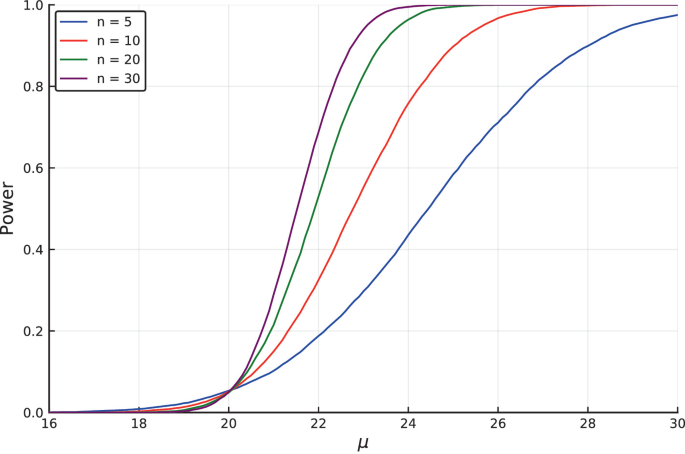
\includegraphics[width=1\linewidth]{overviews/testing-pValues-CIs/figures/one-tailed-power.png}
\end{figure}
\begin{figure}
    \centering
    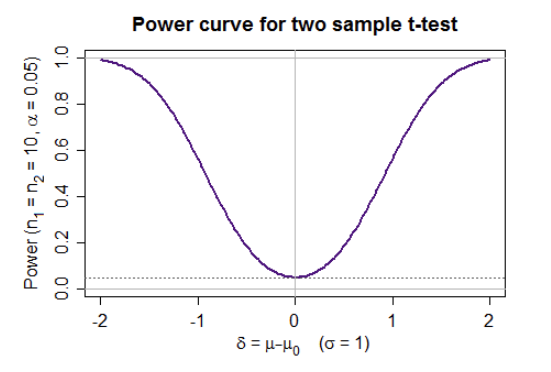
\includegraphics[width=1\linewidth]{overviews/testing-pValues-CIs/figures/two-tailed-power.png}
\end{figure}


\end{document}
